\newpage
{\bfseries МРНТИ 61.51.17}
\hfill {\bfseries \href{https://doi.org/10.58805/kazutb.v.2.23-260}{https://doi.org/10.58805/kazutb.v.2.23-260}}

\sectionwithauthors{D.Zh. Amankeldin, N.U. Nurgaliyev, E.B. Zhunussova, Kh.B.Omarov, A.K. Zhumabekova, Sh.Zh.Ussenkulova,  O.R. Orynbassar}{OPTIMIZATION OF THE OPERATION OF AN ISOMERIZATION INSTALLATION
FOR LIGHT PETROL FRACTIONS}

\begin{center}
{\bfseries \textsuperscript{1}D.Zh. Amankeldin, \textsuperscript{1}N.U. Nurgaliyev, \textsuperscript{1}E.B. Zhunussova, \textsuperscript{1}Kh.B.Omarov, \textsuperscript{1}A.K. Zhumabekova, \textsuperscript{1}Sh.Zh.Ussenkulova, \textsuperscript{2} O.R. Orynbassar}

\textsuperscript{1}Kazakh University of Technology and Business named
after K. Kulazhanov,

Astana, Kazakhstan,

\textsuperscript{2}K. Zhubanov Aktobe Regional State University, Aktobe,
Kazakhstan,

Corresponding author: nurgaliev\_nao@mail.ru
\end{center}

The interest in this process lies in the fact that it has great value
since low-octane components are used as raw materials - the n fraction.
temperature -- 62 °С and catalytic reforming raffinates. This raw
material contains mainly pentane and hexane fractions. This raw
material, as well as fractions С\textsubscript{5} and С\textsubscript{6}
obtained from a gas fractionation unit (GFU), and a central gas
fractionation unit (CGFU), are isomerized in a hydrogen environment in
the presence of a catalyst. Hydrocarbons with a relatively high octane
number are obtained. When isomerizing the pentane fraction, a product
with a higher octane number is obtained. Isomerization of n-pentane is
of interest not only for the oil refining industry, but also for the
petrochemical industry, since isopentane can be converted by
dehydrogenation into isoprene, a raw material for rubber. The article
conducted a study on the selection of the optimal catalyst for the light
gasoline fraction isomerization unit located at the Atyrau Oil Refinery.
The catalytic activity of the catalyst samples was assessed in a
laboratory flow-type installation. Determination of the mass fraction of
С\textsubscript{2}-С\textsubscript{5} hydrocarbons in С\textsubscript{5}
hydrocarbon fractions (in raw materials and catalyst) was carried out by
a method based on the separation of mixture components by gas-liquid
chromatography. The components leaving the chromatographic column were
detected using a thermal conductivity detector. The calculation of the
mass fractions of components was carried out using the normalization
method, taking into account correction factors. The minimum
concentration of C\textsubscript{2}-С\textsubscript{5} hydrocarbons,
determined by the method used, is 0.01-0.05\% wt.

{\bfseries Key words:} isomerization process, catalyst, fraction,
isomerate, chromatographic study, motor gasoline, isomerization unit.

\begin{center}
{\large\bfseries ОПТИМИЗАЦИЯ РАБОТЫ УСТАНОВКИ ИЗОМЕРИЗАЦИИ ЛЁГКИХ БЕНЗИНОВЫХ
ФРАКЦИЙ}

{\bfseries \textsuperscript{1}Д.Ж. Аманкельдин., \textsuperscript{1}Н.У.Нургалиев, \textsuperscript{1}Э.Б. Жунусова, \textsuperscript{1}Х.Б. Омаров,\\ \textsuperscript{1}А.К. Жумабекова, \textsuperscript{1}Ш.Ж. Усенкулова, \textsuperscript{2}Р.О. Орынбасар\textsuperscript{2}}

\textsuperscript{1}Казахский университет технологии и бизнеса
им.К.Кулажанова,

г. Астана, Казахстан,

\textsuperscript{2}Актюбинский региональный университет имени К.
Жубанова, Актобе, Казахстан,

e-mail: nurgaliev\_nao@mail.ru
\end{center}

Интерес к данному процессу заключается в том, что он имеет большую
ценность так, как в качестве сырья используются низкооктановые
компоненты -- фракция н. к. -- 62 ° С и рафинаты каталитического
риформинга. В этом сырье содержится в основном пентановая и гексановая
фракции. Это сырье, а также фракции С\textsubscript{5} и
С\textsubscript{6}, получаемые с газофракционирующей установки (ГФУ), и
центральная газофракционирующая установка (ЦГФУ), изомеризуются в среде
водорода в присутствии катализатора. Получают углеводороды со
сравнительно высоким октановым числом изостроения. При изомеризации
пентановой фракции получают продукт с более высоким октановым числом.
Изомеризация н-пентана представляет интерес не только для
нефтеперерабатывающей, но и для нефтехимической промышленности, так как
изопентан дегидрированием можно превратить в изопрен -- сырье для
каучука. В статье проведено исследование по подбору оптимального
катализатора для установки изомеризации легких бензиновых фракции,
расположенной на Атырауском НПЗ. Оценку каталитической активности
образцов катализатора проводили на лабораторной установке проточного
типа. Определение массовой доли С\textsubscript{2}-С\textsubscript{5}
-углеводородов в С\textsubscript{5}--фракциях углеводородов (в сырье и
катализате) проводили методом, основанном на разделении компонентов
смеси методом газо­жидкостной хроматографии. Фиксирование компонентов,
выходящих из хроматографической колонки, производили с помощью детектора
по теплопроводности. Расчет массовых долей компонентов производили
методом нормирова­ния с учётом поправочных коэффициентов. Минимальная
концентрация углеводородов C\textsubscript{2}-С\textsubscript{5},
определяемая по используемой методике, составляет 0,01-0,05 \% масс.

{\bfseries Ключевые слова:} процесс изомеризации, катализатор, фракция,
изомерат, хроматографическое исследование, автомобильный бензин,
установка изомеризации.

\begin{center}
{\large\bfseries ЖЕҢІЛ БЕНЗИН ФРАКЦИЯЛАРЫН ИЗОМЕРЛЕУ ҚОНДЫРҒЫСЫНЫҢ ЖҰМЫСЫН
ОҢТАЙЛАНДЫРУ}

{\bfseries \textsuperscript{1}Д.Ж. Аманкельдин,
\textsuperscript{1}Н.У.Нургалиев, \textsuperscript{1}Э.Б. Жунусова,
\textsuperscript{1}Х.Б. Омаров,\\
\textsuperscript{1}А.К. Жумабекова, \textsuperscript{1}Ш.Ж. Усенкулова,
\textsuperscript{2}Р.О. Орынбасар}

\textsuperscript{1}Қ.Құлажанов атындағы Қазақ технология және бизнес
университеті,

Астана, Қазақстан,

\textsuperscript{2}Қ.Жұбанов атындағы Ақтөбе өңірлік университеті,
Ақтөбе қаласы, Қазақстан,

e-mail: nurgaliev\_nao@mail.ru
\end{center}

Бұл процеске деген қызығушылық оның құндылығы жоғары, өйткені шикізат
ретінде төмен октанды компоненттер қолданылады-н. к. фракциясы -- 62 °С
және каталитикалық риформинг тазартқыштары. Бұл шикізатта негізінен
пентан және гексан фракциялары бар. Бұл шикізат, сондай-ақ ГФҚ және
ОГФҚ-ден алынған C\textsubscript{5} және C\textsubscript{6} фракциялары
катализатордың қатысуымен сутегі ортасында изомерленеді. Көмір сутектер
изостроенияның салыстырмалы түрде жоғары октан санымен алынады. Пентан
фракциясы изомерленген кезде октан саны жоғары өнім алынады. Н-пентанның
изомерленуі тек мұнай өңдеу үшін ғана емес, сонымен қатар мұнай-химия
өнеркәсібі үшін де қызығушылық тудырады, өйткені сусыздандыру арқылы
изопентанды резеңке үшін изопрен шикізатына айналдыруға болады. Мақалада
Атырау МӨЗ-де орналасқан жеңіл бензин фракцияларының изомерленуін орнату
үшін оңтайлы катализаторды таңдау бойынша зерттеу жүргізілді.
Катализатор үлгілерінің каталитикалық белсенділігін бағалау ағынды
типтегі зертханалық қондырғыда жүргізілді. Көмірсутектердің
С\textsubscript{5} фракцияларындағы (шикізат пен катализатта)
С\textsubscript{2}-С\textsubscript{5}--көмірсутектердің массалық үлесін
анықтау газ--сұйық хроматография әдісімен қоспаның компоненттерін бөлуге
негізделген әдіспен жүргізілді. Хроматографиялық бағаннан шығатын
компоненттерді бекіту жылу өткізгіштік детекторының көмегімен жүзеге
асырылды. Компоненттердің массалық үлестерін есептеу түзету
коэффициенттерін ескере отырып, нормалау әдісімен жүргізілді.
Қолданылатын әдіс бойынша анықталған
C\textsubscript{2}--C\textsubscript{5} көмірсутектерінің ең аз
концентрациясы массалардың 0,01-0,05\% құрайды.

{\bfseries Түйін сөздер:} изомерлеу процесі, катализатор, фракция,
изомерат, хромато-графикалық зерттеу, автомобиль бензині, изомерлеу
қондырғысы.

\begin{multicols}{2}
{\bfseries Introduction.} Large hydrocarbon deposits are located in the
territory of the Caspian Sea, which are characterized by special
geostrategic, geographical, military and political features. In addition
to oil and gas resources, the location between the main markets in the
West and East is of great strategic importance {[}1{]}. The ways of
realization of Kazakhstan oil today depend on complex processing of
productions, where oil is a raw material for the final product. This is
due to the fact that the capacities and technological equipment of the
relevant refineries are not oriented to extract the full range of
products contained in the feedstock {[}2{]}.

Crude oil is a complex raw material from which a wide range of petroleum
products can be obtained. According to the technological schemes of
production, processing into fuel, oil and mixed directions prevails
{[}3{]}. The introduction of the process of isomerization of
straight-run gasoline fractions into the practice of oil refineries
determines the relevance of studying this process, as well as the need
for scientific research in the field of development of technology of
isomerization processes and selection of catalysts that provide optimal
conditions for isomerization reactions {[}4{]}.

The catalysts used in various isomerization technologies have a common
kinetic pattern: at high temperatures, the yield of isoalkanes is
limited by thermodynamic equilibrium, and at low temperatures, the
reaction rate decreases. The selection of a catalyst that provides a
minimum yield of aromatic compounds and olefins is important {[}5{]}.

The purpose of isomerization processes in oil refining is to improve the
anti-knock properties of aviation and motor gasoline. In the oil
refining industry, they began to be used to produce isobutane from
\emph{n}-butane. Isobutane was further alkylated with butylenes to give
2,2,4-trimethylpentane (isooctane).

The great value of the isomerization process lies in the fact that
low-octane components are used as raw materials - the n fraction.
temperature -- 62 °С and catalytic reforming raffinates. This raw
material contains mainly pentane and hexane fractions. This raw
material, as well as fractions С\textsubscript{5} and С\textsubscript{6}
obtained with HFCs and CHFCs, are isomerized in a hydrogen environment
in the presence of a catalyst. Hydrocarbons with a relatively high
octane number are obtained. When isomerizing the pentane fraction, a
product with a higher octane number is obtained. Isomerization of
n-pentane is of interest not only for the oil refining industry, but
also for the petrochemical industry, since isopentane can be converted
by dehydrogenation into isoprene, a raw material for rubber. Thus,
isomerization can serve both for the production of high-octane gasoline
and for the production of valuable synthetic rubbers {[}6,7{]}.

The isomerization of paraffin hydrocarbons on a solid catalyst proceeds
in two directions: hydrogenation-dehydrogenation and isomerization
itself. When a hydrocarbon molecule reaches the catalyst, one of the
hydrogen atoms of that molecule is adsorbed on the metal site, and the
associated carbon atom is adsorbed on the acid site. The adsorbed
molecule isomerizes and leaves the catalytic surface under the action of
molecular hydrogen {[}8-10{]}.

Catalysts can be divided into five main groups: Friedel-Crafts
catalysts, tungsten sulfide, bifunctional catalysts, synthetic noble
metal zeolites (including rare earth metal additives) and complex
catalysts (combining bifunctional and zeolite catalysts with
Friedel-Crafts catalysts).

Friedel-Crafts catalysts in most cases contain anhydrous aluminum
chloride (sometimes with antimony trichloride) in the form of a complex
with hydrocarbons activated by hydrogen chloride. Isomerization using
Friedel-Crafts catalysts can be carried out at 20 \emph{atm} and 40-120
°C and even at 24-50°C (catalysts based on bromine chloride).

Tungsten sulfide from sulfide catalysts turned out to be most active and
selective at moderate reaction temperatures (about 400 °C). The degree
of isomerization of c-hexane on it reached 60\% with insignificant
hydrocarbon splitting. To ensure stable operation of the catalyst in the
system, it is necessary to maintain a pressure of at least 40 atm.

It is important to note that the presence of naphthenic hydrocarbons (up
to 20-25\%), sulfur compounds and moisture in the raw material does not
deteriorate the process performance. The use of hydrogen, despite the
fact that it inhibits the isomerization reaction on tungsten sulfide, is
necessary because it prevents coking of the catalyst {[}11{]}.

Bifunctional catalysts are a type of reforming catalyst - platinum or
palladium on alumina. However, sometimes aluminosilicate or a mixture of
aluminum and boron oxide is used as a carrier. These catalysts have
sufficient selectivity for the isomerization of
С\textsubscript{5}-С\textsubscript{6} paraffinic hydrocarbons, which
distinguishes them from Friedel-Crafts catalysts, but their activity is
very low, so the temperature has to be increased

Increasing the acidity of a bifunctional catalyst is also achieved by
treating it with chlorine-containing organic compounds, and maintaining
acidity by introducing HC1 into the system {[}12{]}.

Synthetic zeolites with noble metals - platinum or palladium, as well as
with additives of rare earth metals are based on the use of crystalline
aluminosilicates - zeolites. These catalysts are very active in the
isomerization of n-peitane and n-hexane. Platinum or palladium deposited
on Y-type zeolite allows the isomerization process to be carried out at
315-343 °C, i.e. approximately 150°C lower than when using alumina as a
carrier. Experiments on catalysts with different platinum contents
showed that even a minimal concentration of platinum ensures high
efficiency of isomerization of paraffinic hydrocarbons. Typically the
platinum or palladium content ranges from 0.3 to 0.6\% {[}13{]}.

Complex catalysts combine the advantages of bifunctional and zeolite
catalysts (often called hydroisomerization catalysts) with the
advantages of Friedel-Crafts catalysts, which allow the process to be
carried out at lower temperatures. Complex catalysts can be used at
90-200 °C. With their help, almost equilibrium yields of isopentanes and
isohexanes are achieved. Their selectivity is high: only a small amount
of C\textsubscript{1}-С\textsubscript{4} paraffins is formed as a
by-product. However, it should be borne in mind that aluminum chloride,
which is usually included in complex catalysts, is hygroscopic; sooner
or later it hydrolyzes, and the resulting aluminum hydroxide is
deposited inside the pores of the catalyst, reducing their volume and
complicating regeneration. In this regard, complex catalysts have not
found application in isomerization processes carried out at oil
refineries {[}14-16{]}.

Recently, platinum treated with chlorine-containing organic compounds
has been used as a catalyst. The activity of the catalyst is maintained
by additional input of HC1, as well as by a gradual increase in
temperature to 160 °C.

For the first time, this work proposes replacing the proprietary UOP
1-8+/UOP I-82 catalyst (USA) with a less expensive SI-2 catalyst
{[}17{]}. This catalyst allows the isomerization process to be carried
out at the inlet of reactors with a high degree of isomerization of both
pentanes and hexanes. It consists of platinum evenly distributed over
the surface of sulfated zirconium oxide modified with aluminum. It has
high activity in the isomerization reactions of low-boiling hydrocarbons
under thermodynamically favorable conditions, not inferior in efficiency
to chlorinated catalysts {[}17{]}. At the same time, its resistance to
catalytic poisons is higher, and it also tolerates their short-term
breakthroughs without reducing activity {[}18{]}. In addition,
additional advantages of such catalysts are their long service life (up
to 10 years) and the possibility of regeneration.

{\bfseries Materials and methods.} The catalytic activity of the SI-2
catalyst samples was assessed in a laboratory flow-type installation
(Figure 1).

The normal pentane fraction from the raw material tank is drained by
gravity into a dosing pump, from where it is dosed into the evaporator.
The recycle fraction of normal pentane is similarly fed through a
parallel feed dosing line. Gas streams of fresh (concentrated) and
recycle fractions are mixed with each other and with hydrogen and sent
to the reactor. The catalyst is loaded into the reactor in a stationary
bed. The reactor is placed in a laboratory furnace, which heats the
reaction stream to the reaction temperature.
\end{multicols}

\begin{figure}[H]
	\centering
	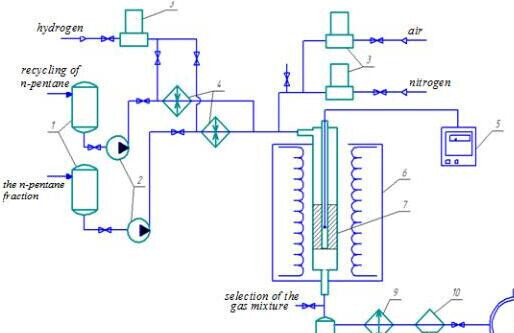
\includegraphics[width=0.6\textwidth]{assets/1053}
	\caption*{Figure 1 - Diagram of a laboratory setup for testing a catalyst in the process of isomerization of n-pentane to isopentane:}
	\caption*{1 -- containers for raw materials; 2 -- dosing pumps; 3 -- gas flow meters; 4 -- raw material evaporators; 5 -- temperature meter; 6 -- laboratory single-zone furnace; 7 -- laboratory reactor; 8 -- separator; 9 -- catalytic condenser; 10 - catlysate separator; 11 -- drum type gas meter}
\end{figure}

\begin{multicols}{2}
In the catalyst layer, pentane of normal structure is isomerized into
pentane of iso-structure. The reaction products are sent to a separator,
in which the mixture of C\textsubscript{5} hydrocarbons is condensed.
The gas part of the flow, consisting mainly of hydrogen and partly of
cracking products, is taken into account in a drum gas meter.

The catalyst is loaded into a pre-prepared reactor. A catalyst with a
volume of 10 ml is loaded into an isothermal reactor, and palladium is
reduced in a hydrogen flow of 375 h\textsuperscript{-1} at a temperature
of 145 °C and a pressure of 1 atm for 1 hour.

Determination of the mass fraction of
C\textsubscript{2}--C\textsubscript{5} hydrocarbons in C5 hydrocarbon
fractions (in raw materials and catalyst) was carried out by a method
based on the separation of mixture components by gas-liquid
chromatography. The components leaving the chromatographic column were
detected using a thermal conductivity detector.

The calculation of the mass fractions of components was carried out
using the normalization method, taking into account correction factors.
The minimum concentration of C\textsubscript{2}--C\textsubscript{5}
hydrocarbons, determined by the method used, is 0.01-0.05 \% wt.

The preparation of the stationary phase and filling of the
chromatographic column was carried out as follows. Diatomite brick was
ground in a mortar, sifted on sieves with opening sizes of 0.16 and 0.25
mm, selecting a fraction of 0.16-0.25 mm, it was poured with
concentrated nitric acid in an evaporation (porcelain) cup and kept
under the acid for 3 hours. After that, the diatomite brick was washed
from the acid with distilled water until a neutral reaction (the last
portion of water should not cause a change in the color of methyl
orange).

The washed diatomite was dried at a temperature of 100-120 °C for 1 hour
and calcined at a temperature of 900 °C for 3 hours. Cooling was carried
out in a desiccator, after which it was again sieved through sieves with
opening sizes of 0.16 and 0.25 mm.

The prepared diatomite brick (chamotte) was impregnated with a
stationary phase - triethylene glycol dibutyrate in an amount of 15-20\%
by weight of diatomite. A sample of 15--20 g of triethylene glycol
dibutyrate was measured into a beaker with a capacity of 250
cm\textsuperscript{3} on a laboratory scale, dissolved in 200
cm\textsuperscript{3} of ethyl ether and transferred quantitatively into
a round-bottomed flask with a capacity of 500 cm\textsuperscript{3}. 100
g of prepared diatomite (chamotte) was poured into the solution. The
mixture was mixed well and kept for 20--30 minutes. The flask was sealed
with a stopper with two siphons for purging, and the contents were
shaken for an additional 5--6 minutes. Ethyl ether was distilled off in
a water bath at a temperature of 35--40 °C with simultaneous purging
with nitrogen until the smell of ethyl ether disappeared.

Before filling the chromatographic column with the finished sorbent, the
column was washed successively with ethyl alcohol, acetone and then
purged with air pressure for 20 minutes. A clean and dry column was
filled with the prepared stationary phase using a funnel and a water jet
(oil) pump. One of the ends of the column was previously covered with a
glass wool swab and connected to the pump. The nozzle was compacted with
a vibrator. The column was also tapped with a wooden stick to compact
it. The other end of the column was also covered with a glass wool swab.

Chromatographic analysis was carried out under the following conditions:

Column temperature, °C 20--40

Chromatograph operating mode isothermal

Carrier gas speed, cm\textsuperscript{3}/min 25--30

Chart tape speed, mm/hour 240--720

Объём вводимой жидкой пробы, mkl 2--3

Volume of injected vapor-gas mixture, cm\textsuperscript{3} 1--2

The identification of components С\textsubscript{2}-С\textsubscript{5}
in the hydrocarbon mixture using the chromatogram was carried out taking
into account the relative retention volumes given in Table 1.

\begin{table}[H]
\caption*{Table 1 -- Relative retention volumes of raw material components on a 15\% dibutyrate triethylene glycol column on diatomite brick and sensitivity correction factors for the thermal conductivity detector}
\centering
\begin{tabular}{|l|l|l|}
\hline
Component name & Vrel. & K \\ \hline
Ethane + ethylene & 0,01 & 0,8 \\ \hline
Carbon dioxide & 0,02 & 1,36 \\ \hline
Propane & 0,04 & 0,92 \\ \hline
Propylene & 0,06 & 0,92 \\ \hline
Isobutane & 0,09 & 1,02 \\ \hline
n-Butane & 0,13 & 1 \\ \hline
Butene-1 + isobutylene & 0,18 & 1,01 \\ \hline
Butene-2 – trans & 0,23 & 0,99 \\ \hline
Butene-2-cis & 0,27 & 1,01 \\ \hline
Isopentane & 0,29 & 1,07 \\ \hline
Butadiene & 0,32 & 1,02 \\ \hline
3-methylbutene-1 & 0,33 & 1,11 \\ \hline
n-Pentane & 10,38 & 1,05 \\ \hline
\end{tabular}
\end{table}

The peak area of all components was calculated as the product of the
peak height and its width, measured at half the height (half-width). The
resulting value of the area of each peak was multiplied by the
sensitivity scale of the device. The location of the peaks on the
chromatographic diagram is shown in Figure 2.
\end{multicols}

\begin{figure}[H]
	\centering
	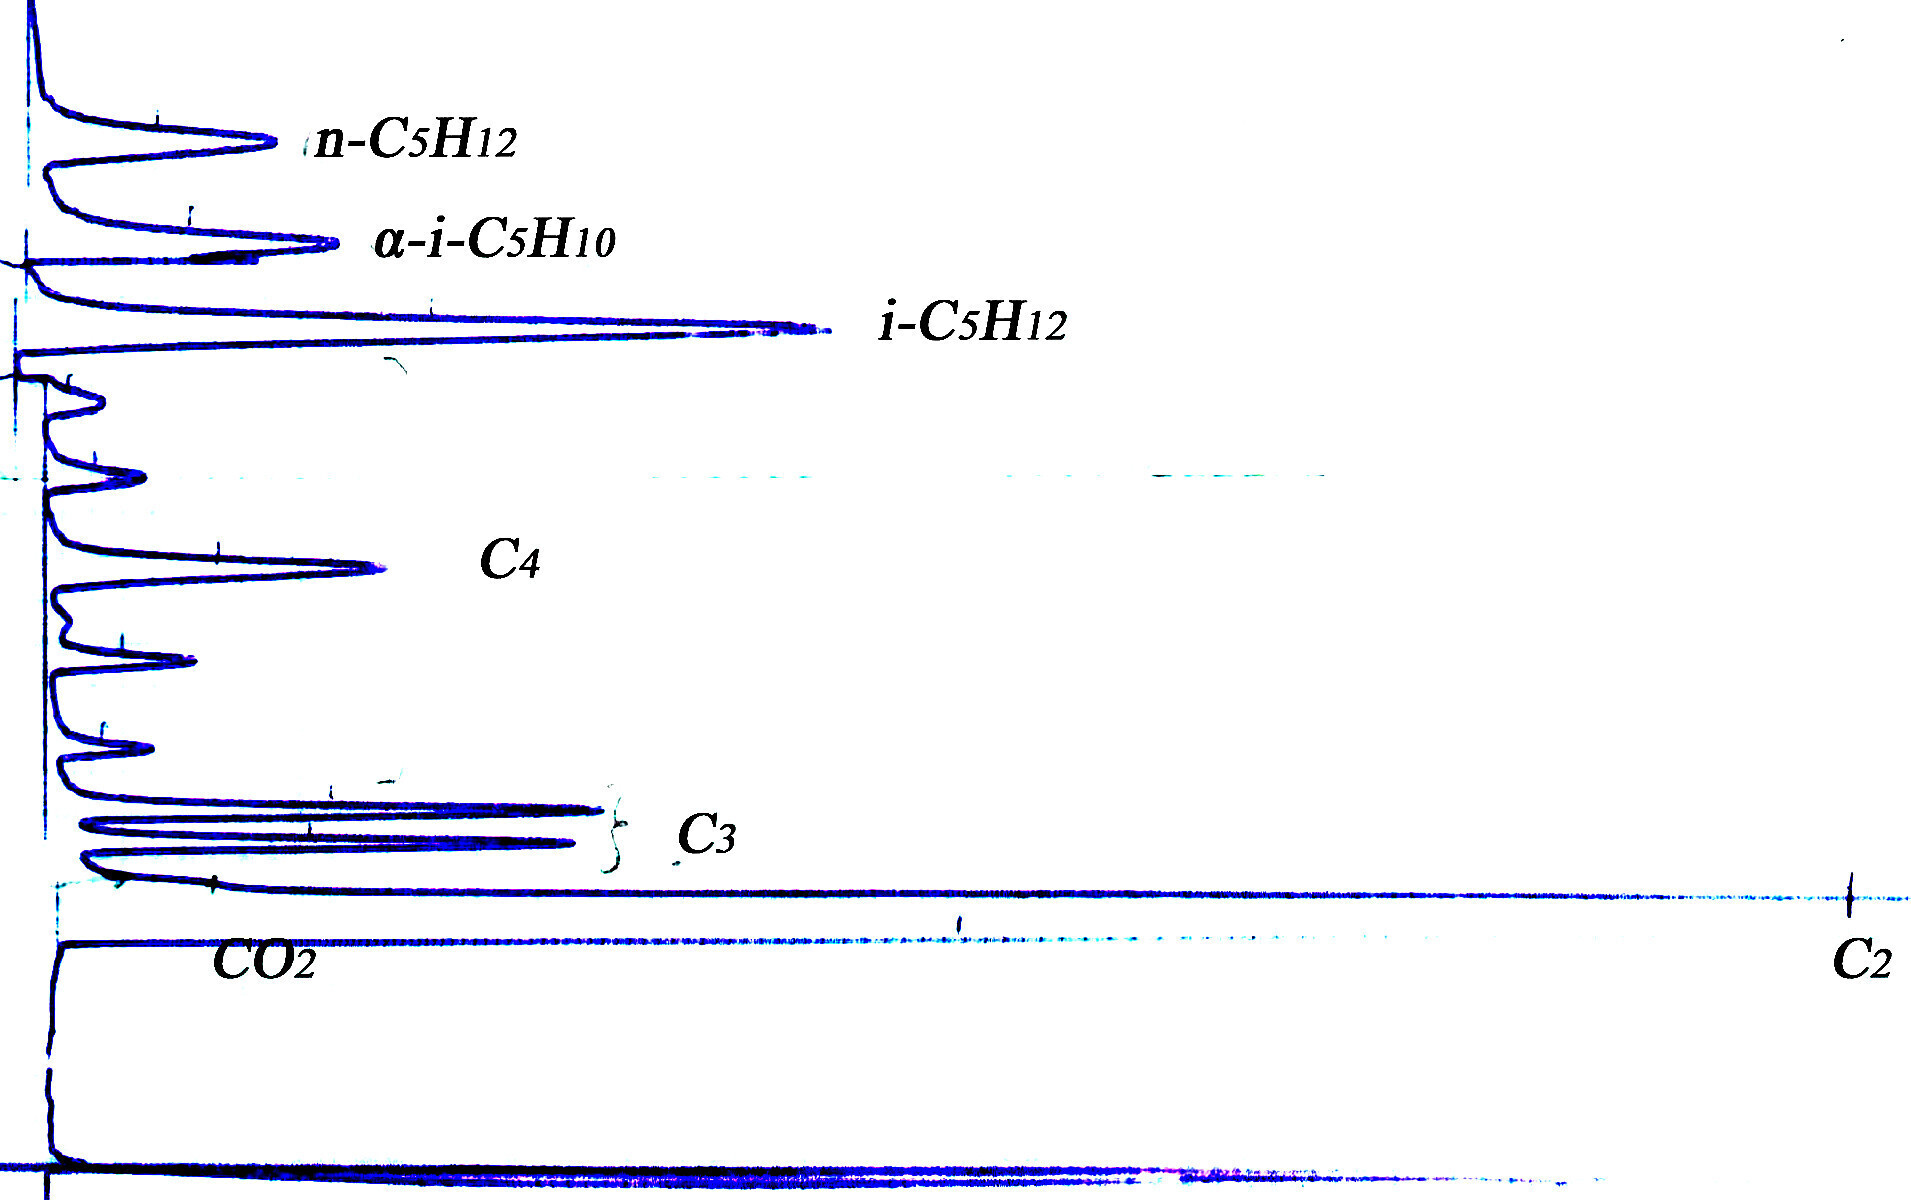
\includegraphics[width=0.5\textwidth]{assets/1054}
	\caption*{Figure 2 -- Location of the chromatographic response of each component on the diagram}
\end{figure}

\begin{multicols}{2}
The volume fraction of each component in the contact gas (X) in percent
was calculated using the formula:

\[X_{i} = \frac{K_{i} \times S_{i} \left( 100 - \sum X \right)}{\sum (S_{i} \times K)} \]

где K is the molar correction factor of the component (Table 1);
S\textsubscript{i} - component peak area,\\
cm\textsuperscript{2}, ∑S\textsubscript{i} - sum of the areas of all
components multiplied by correction factors, cm\textsuperscript{2}, ∑Х -
the sum of the volume fractions of the components of permanent gases,
determined by the method of analysis of Н\textsubscript{2},
О\textsubscript{2}, N\textsubscript{2}, CH\textsubscript{4} CO in the
composition of the contact gas.

The result of the analysis is taken as the result of one determination.

From the data of gas chromatographic analysis, the conversion of
n-pentane and the selectivity of isopentane formation are calculated.

{\bfseries Results and discussion.} Table 2 presents the results of
isomerization of the pentane-hexane fraction with an estimate of the
yield of isopentane.
\end{multicols}

\begin{table}[H]
\caption*{Table 2 -- Effect of temperature on the yield of isomerization products on the SI-2 catalyst (space velocity of the raw material in liquid 1.5 h-1)}
\centering
\begin{tabular}{|l|l|l|l|}
\hline
Test temperature, \tsp{о}С & Isopentane yield, \% & Selectivity, \% & Equilibrium concentration of isopentane, \% \\ \hline
110 & 27,4 & 99,1 & 42 \\ \hline
120 & 30,8 & 99 & 39 \\ \hline
130 & 33,5 & 99 & 37 \\ \hline
140 & 35,9 & 89,7 & 35 \\ \hline
150 & 33,1 & 89,7 & 34 \\ \hline
170 & 30,2 & 89,1 & 31 \\ \hline
\end{tabular}
\end{table}

\begin{multicols}{2}
As can be seen from Table 2, the highest yield of isopentane with a
selectivity of 89.7 \% is observed at a temperature of 140
\textsuperscript{о}C.

Table 3 shows the effect of space velocity on the yield of isopentane.
As can be seen from the table, the most effective space velocity is 1.0
h-1, at which an increase in isopentane yield to 36.4 \% and selectivity
to 89.8 \% is achieved.
\end{multicols}

\begin{table}[H]
\caption*{Table 3 -- Effect of space velocity on the yield of isomerization products on the SI-2 catalyst (process temperature 140 \textsuperscript{о}С)}
\centering
\begin{tabular}{|l|l|l|}
\hline
Volumetric velocity of raw materials (liquid), hour-1 & Isopentane yield, \% & Selectivity, \% \\ \hline
1.0 & 36.4 & 89.8 \\ \hline
1.5 & 35.9 & 89.7 \\ \hline
2.0 & 30.1 & 89.0 \\ \hline
\end{tabular}
\end{table}

\begin{multicols}{2}
In addition to pentane isomerization, it is necessary to evaluate the
yields of isohexane. Figure 3 shows the results of a study of the
dependence of the isomerate yield on temperature (for comparison,
production data for the operating catalyst I-82 are presented).
\end{multicols}

\begin{figure}[H]
	\centering
	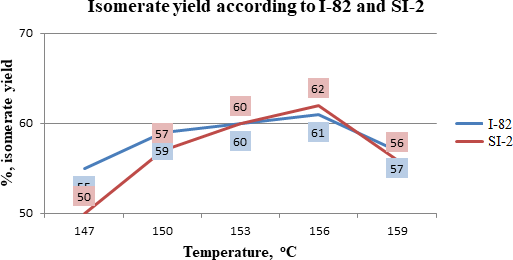
\includegraphics[width=0.6\textwidth]{assets/1056}
	\caption*{Figure 3 - Ratio of isomerate yield to temperature}
\end{figure}

\begin{multicols}{2}
As can be seen from the graph of the dependence of isomerizate yield on
temperature, the highest isomerizate yield is observed on the SI-2
catalyst (62 \%) at a temperature of 156 \textsuperscript{о}C, at which
the isomerizate yield on the I-82 catalyst was 61 \%.

Figure 4 shows octane number data at various temperatures (for
comparison, production data for the current I-82 catalyst is presented).
\end{multicols}

\begin{figure}[H]
	\centering
	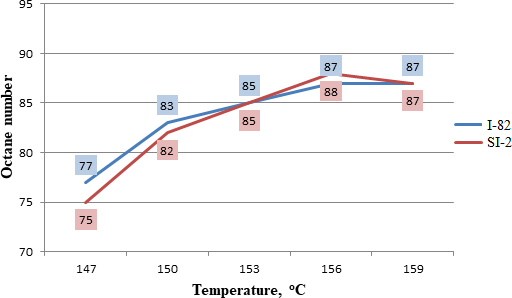
\includegraphics[width=0.6\textwidth]{assets/1057}
	\caption*{Figure 4 - Ratio of octane number to temperature}
\end{figure}

\begin{multicols}{2}
As can be seen from Figures 3 and 4, catalysts SI-2 and I-82 at the same
temperature ranges show almost identical performance.

{\bfseries Conclusions.} Thus, the catalytic activity of the SI-2 catalyst
was evaluated at the light gasoline fractions isomerization unit. A
feature of this catalyst is its high isomerizing activity, which is
practically not inferior to chlorinated aluminum oxide catalysts with
significant resistance to the effects of catalytic poisons {[}18{]}. As
a result of the study of the process of isomerization of light gasoline
fractions on the SI-2 catalyst, it was revealed that the catalytic
performance of the proposed SI-2 catalyst and the I-82 catalyst used in
production have almost the same performance. It is necessary to take
into account that the cheaper SI-2 catalyst has many of the above
effective properties.
\end{multicols}
\newpage
\begin{center}
{\bfseries References}
\end{center}

\begin{noparindent}
1. Umirova G.K., Suleimenov A.O. The use of special high-tech
geophysical equipment (hitech) in the analysis of mechanical
characteristics, anisotropy and fracturing of rocks on the example of
the southern part of the Zhanazhol field // Bull. Satbayev Univ.,
2021.-Vol. 5.- P. 24-38. DOI~https://doi.org/10.51301/vest.su.2021.i5.04

2. Satayeva, S.S., Jubanaliyeva, A.M. Purification of hydrocarbon raw
materials of oil field Zhanazhol from methyl-and ethylmercaptane //
Bulletin of the L.N. Gumilyov Eurasian National University, 2018. --
Vol.124 (3).- P.14-18. DOI 10.32523/2616-6771-2018-124-3-14-18

3.Baidauletova L.R., Bukanova A.S., Orazova G.A. Technological methods
for obtaining petrochemical products // Bull. Atyrau Univ., 2018.-Vol.
48 (1).- P. 155--158.

4. Kaldygozov E., Sydyk D., Tleubayeva E., Abdikerimov B. Karashyganak
oil and gas condensat processing variant for production of commodity oil
products // Indust. Techn. Engin., 2018. - Vol. 4.- P.65-69.

5. Jiang X., Long F., Cao X., Zhao J., Liu P., Xu J. Catalytic cracking
of waste cooking oil followed with hydro-isomerization for high-quality
biofuel production // J. Clean. Prod., 2022. -- Vol. 345:131027.

https://doi.org/10.1016/j.jclepro.2022.131027.

6. Zhuravleva M. V., Klimentova G. Ju., Zinnurova O. V., Goncharova I.
N., Firsin A. A.Kataliticheskie processy neftehimii i neftepererabotki:
uchebnoe posobieZhuravleva M.V., /Minobrnauki Rossii, Kazan. nats.
issled. tekhnol. un-t. - Kazan\textquotesingle: Izd-vo KNITU, 2019. -316
s. {[}in Russ.{]}

7. Il\textquotesingle in A.V., Davletshin R.R., Kuramshin A.I.
Khimicheskaya tekhnologiya neft\textquotesingle{} i ee pererabotka:
uchebnoe posobie. -- Minobrnauki Rossii, Kazan. nats. issled. tekhnol.
un-t.-Kazan\textquotesingle: Izd-vo KNITU, 2018.- 80 s. {[}in Russ.{]}

8. Arslanov A. N., Abdullin A. I. Perspektivy razvitiya protsessa
izomerizatsii/ Vestnik tekhnologicheskogo universiteta. 2015. --
T.18(9)-.S. 39-40. {[}in Russ.{]}

9. Kuz\textquotesingle mina R.I., Frolov M.P., Liventsev V.T.
Izomerizatsiya -- protsess polucheniya ekologicheski chistykh benzinov:
uchebnoe posobie po kursam «Khimiya nefti i gaza», «Khimicheskaya
tekhnologiya motornykh topliv i uglerodnykh materialov.-Saratov:
Saratovkii gosudarstvennyi universitet, 2008.- 88 s. {[}in Russ.{]}

10. Solov\textquotesingle ev A.S. Tekhnologiya polucheniya komponenta
benzinov s ponizhennym soderzhaniem benzola i

aromaticheskikh
uglevodorodov S\textsuperscript{9+} na osnove riformata. Avtoreferat
diss. \ldots{} kand. tekhn. nauk. Ufa, 2003.-24 s. {[}in Russ.{]}

11. GOST 32513-2013 Topliva motornye. Benzin neetilirovannyi.
Tekhnicheskie usloviya.- M.: Standartinform, 2013.- 12 s. {[}in Russ.{]}

12. Kostenko A.V. Osvoenie nizkotemperaturnogo protsessa izomerizatsii
legkikh benzinovykh fraktsii «Izomalk--2» / A.V. Kostenko, M.M. Goev,
E.V. Ferkel\textquotesingle, L.I. Solovykh, A.N. Shakun, M.L. Fedorova
// Neftepererabotka i neftekhimiya. Nauchno--tekhnicheskie dostizheniya
i peredovoi opyt. -2006. -№ 2. {[}in Russ.{]}

13. Gartman V.L. Promyshlennye katalizatory riforminga uglevodorodov i
tendentsii ikh optimizatsii / V.L. Gartman, A.V. Obysov, A.V.
Dul\textquotesingle nev // Kataliz v promyshlennosti.-2007.- № 5. - S.
37-42. {[}in Russ.{]}

14. Khimicheskaya tekhnologiya. Pererabotka nefti i gaza: uchebnoe
posobie: uchebnoe posobie/ - Almaty: TOO "Izdatel\textquotesingle stvo
Bastau", 2018. -- 260 c. {[}in Russ.{]}

15. Igumnov A.S. Variant sovershenstvovaniya ustanovki izomerizatsii
benzinovykh fraktsii // Sovremennye naukoemkie tekhnologii, 2013.- №
6.-S. 193. (in Russ).

16. Chuzlov V. A. Sovershenstvovanie protsessa izomerizatsii
pryamogonnykh benzinovykh fraktsii na stadiyakh kataliticheskogo
prevrashcheniya i rektifikatsii. Avtoreferat diss. \ldots{} kand. tekhn.
nauk. Tomsk, 2018. - 20 s. {[}in Russ.{]}

17. Fedorov Yu. A., Dmitriev Yu.K. Sovershenstvovanie ustanovki
izomerizatsii na OOO «Gazprom neftekhim Salavat» // Bulatovskie
chteniya, sbornik statei, 2018.- S.310-313. {[}in Russ.{]}

18. Kazantsev E.O. Analiticheskii obzor katalizatorov izomerizatsii
legkoi benzinovoi fraktsii // Vestnik magistratury, Ser. Khimicheskie
nauki, 2019. -№ 1-2(88).- S. 17-22. {[}in Russ.{]}
\end{noparindent}

\emph{{\bfseries Information about authors:}}

\begin{noparindent}
Amankeldin D.Zh.-Master\textquotesingle s Student, Specialty «Oil and
Gas Business», Kazakh University of Technology and Business named after
K.Kulazhanov, Astana, Kazakhstan, e-mail: a\_daniyar94@mail.ru;

Nurgaliyev N.U. -Candidate of Chemical Sciences, Associate Professor,
Kazakh University of Technology and Business named after K.Kulazhanov,
Astana, Kazakhstan, е-mail: nurgaliev\_nao@mail.ru;

zhunussova e.B.-Candidate of Technical Sciences, Associate Professor,
Kazakh University of Technology and Business named after K.Kulazhanov,
Astana, Kazakhstan, е-mail: tahmina.66@mail.ru;

Omarov K.B.-Doctor of Technical Sciences, Professor, Kazakh University
of Technology and Business named after K.Kulazhanov, Astana Kazakhstan,
, e-mail: homarov1963@mail.ru;

Zhumabekova A.K.-Candidate of chemical sciences, Associate Professor,
Kazakh University of Technology and Business named after K.Kulazhanov,
Astana, Kazakhstan, e-mail: zhumabekova\_ak@mail.ru;

Ussenkulova Sh.Zh.-Doctor of PhD, Kazakh University of Technology and
Business named after K.Kulazhanov, Astana, Kazakhstan, e-mail:
sholpan\_\_1990@mail.ru;

Orynbassar R.O. - Candidate of chemical sciences, Associate Professor,
K.Zhubanov Aktobe Regional State University, Aktobe, Kazakhstan, е-mail:
orynbassar.raigul@gmail.com.
\end{noparindent}

\emph{{\bfseries Сведения об авторах}}

\begin{noparindent}
Аманкельдин Д.Ж.-магистрант, Казахский университет технологии и бизнеса
им. К.Кулажанова, Астана, Казахстан, e-mail: a\_daniyar94@mail.ru;

Нургалиев Н.У.-кандидат химических наук, ассоциированный профессор,
Казахский университет технологии и бизнеса им. К.Кулажанова, Астана,
Казахстан, e-mail: nurgaliev\_nao@mail.ru;

Жунусова Э.Б. - кандидат технических наук, ассоциированный профессор,
Казахский университет технологии и бизнеса им. К.Кулажанова, Астана,
Казахстан, e-mail: tahmina.66@mail.ru;

Омаров Х. Б.-доктор технических наук, профессор, Казахского университета
технологии и бизнеса имени К.Кулажанова, Астана, Казахстан, e-mail:
homarov1963@mail.ru;

Жумабекова А.К.-кандидат химических наук, ассоциированный профессор,
Казахский университет технологии и бизнеса им. К.Кулажанова, Астана,
Казахстан, e-mail: zhumabekova\_ak@mail.ru;

Усенкулова Ш.Ж.- доктор PhD, ассоциированный профессор, Казахский
университет технологии и бизнеса им. К.Кулажанова, Астана, Казахстан,
e-mail: sholpan\_\_1990@mail.ru;

Орынбасар Р.О.-кандидат химических наук, ассоциированный профессор,
Актюбинский региональный университет имени К. Жубанова, Актобе,
Казахстан, е-mail: orynbassar.raigul@gmail.com.
\end{noparindent}
